		  
A state diagram is an event-based modeling which used to represent the condition of the system or part of the system at finite instances of time. It's a behavioral diagram and it represents the behavior using finite state transitions.


\begin{figure}[H]
\begin{center}	

	\tcbox{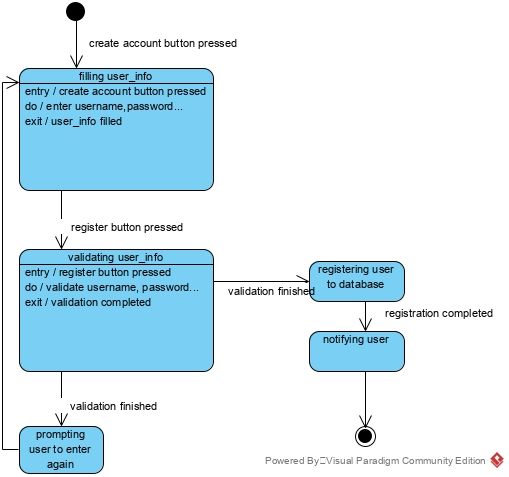
\includegraphics[width=15cm]{Diagram/state/Create Account.png}}
	\caption{State diagram for creating account.}
	\label{dia_stt_crtacnt}

\end{center}
\end{figure}

\begin{figure}[H]
\begin{center}	

	\tcbox{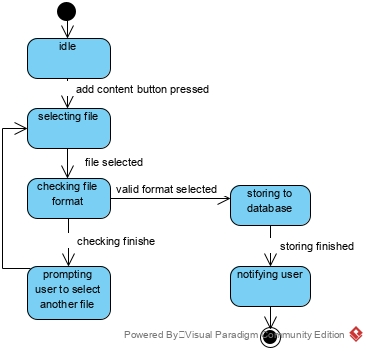
\includegraphics[width=10cm]{Diagram/state/Add Content.png}}
	\caption{State diagram for adding content.}
	\label{dia_stt_addcntnt}

\end{center}
\end{figure}

\begin{figure}[H]
\begin{center}	

	\tcbox{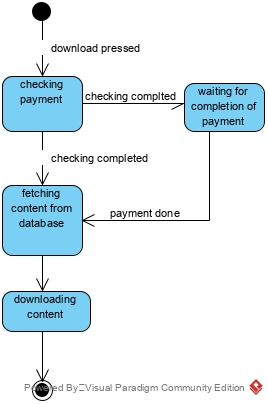
\includegraphics[width=10cm]{Diagram/state/Download Content.png}}
	\caption{State diagram for downloading content.}
	\label{dia_stt_dwnldcntnt}

\end{center}
\end{figure}

\begin{figure}[H]
\begin{center}	

	\tcbox{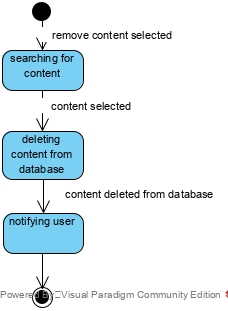
\includegraphics[width=8cm]{Diagram/state/Remove Content.png}}
	\caption{State diagram for removing content.}
	\label{dia_stt_rmvcntnt}

\end{center}
\end{figure}